\section{Entendiendo el Modelo Entidad – Relación}
\subsection*{i. }

\addcontentsline{toc}{subsection}{d.}
\textbf{A continuación, se muestran tres representaciones posibles referidas a las relaciones entre Sitios de taxis, Choferes y Taxis. Analiza las ventajas y desventajas de cada propuesta, contestando las preguntas que se presentan a continuación:}
\begin{enumerate}
    \item \textbf{Indica qué diagramas representan la información requerida por las siguientes solicitudes de información:}

    \textbf{¿Qué taxis maneja el chofer Raúl López en el sitio Santa Fe?}

    El diagrama a) no puede contestar satisfactoriamente esta consulta, pues aunque un chofer puede tener un taxi en un sitio, no sabemos si el chofer lo maneja; por ejemplo, podemos saber que Raúl López tiene un taxi rojo en el sitio Santa Fe, pero no sabemos si lo maneja él. Por otro lado, el diagrama b) tampoco lo puede satisfacer, pues sabes qué chofer maneja qué taxi, pero no sabes si lo maneja en ese sitio; solo sabes que el taxi tiene sitio, pero no si lo maneja allí; por ejemplo, el chofer Raúl López maneja un carro rojo y ese carro rojo tiene sitio en Santa Fe, pero no sabemos si Raúl López lo maneja en Santa Fe. Finalmente, el diagrama c) sí lo satisface, pues precisamente la agregación asocia a cada chofer con la relación Manejar a un par exacto (Sitio, Taxi). Así, si Raúl López maneja un taxi (digamos rojo) que pertenece al sitio Santa Fe, como el par ya está hecho como un todo, se sabe que es en ese sitio específico.

    \textbf{¿A qué sitios está afiliado el chofer Carlos Reyes?}

    Claramente el diagrama a) lo satisface, pues te permite asociar a cada chofer con un sitio y un taxi mediante la relación Tener, así que podemos conocer a qué sitios está asociado el conductor Carlos Reyes. Sin embargo, ni el diagrama b) ni el c) satisfacen conocer a qué sitio está afiliado. En el diagrama b), Carlos Reyes puede manejar el taxi rojo y ese taxi tiene sitio, pero al carecer de una relación directa entre chofer y sitio, no se sabe si Carlos Reyes tiene sitio (o está afiliado) de forma independiente. Asimismo, en el diagrama c), un chofer maneja un par (Sitio, Taxi); sin embargo, si el chofer no maneja activamente, no sabemos si está asociado al sitio o no.

    \textbf{¿Qué taxis están asociados al sitio Universidad?}

    En este caso, los 3 diagramas me pueden dar a conocer qué taxis están asociados al sitio Universidad, ya que todos cuentan con la relación Tener, la cual asocia directamente a la entidad Taxi con la entidad Sitio. Así, resta encontrar las parejas que tengan en la posición de sitio a Universidad y un taxi distinto en cada uno (se puede notar que el diagrama a) causa un poco de redundancia, pues además asocia al chofer con ellos, cosa que trae repeticiones en las parejas de Taxi y Sitio).

    \item \textbf{¿Qué modificación harías en el diagrama de la figura a), sin perder información, para que se puedan conocer qué taxis maneja cada chofer?}

    En este caso, para no perder información, es suficiente agregar una relación binaria directa entre Chofer y Taxi llamada Manejar y mantener la relación Tener. Con ello podríamos saber además qué chofer maneja qué taxi. El diagrama se muestra en la siguiente figura:
    \begin{figure}[H]
        \centering
        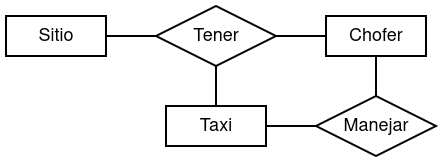
\includegraphics[width=0.6\textwidth]{imagenes/a)manejar.png}
        \caption{Diagrama actualizado con la relación Manejar.}
    \end{figure}

    \item \textbf{¿Qué diferencia existe entre los diagramas de las figuras a) y c)?}

    La diferencia más obvia a primera vista, como se notó en la primera pregunta, es que el diagrama a) no nos permite saber qué chofer maneja qué taxi, mientras que el diagrama c) sí lo hace. Sin embargo, la distinción estructural más relevante es que el inciso a) ubica a todas las entidades al mismo nivel, por lo que aun si pudiera asociar a un taxi y un chofer, no da información al mismo tiempo sobre en qué sitio lo maneja; mientras que el diagrama c) utiliza la abstracción de agregación para empaquetar el par (Sitio, Taxi). Esto nos permite conocer qué chofer maneja un taxi en un sitio determinado.

    \item \textbf{Cómo modificarías el diagrama de la figura a) para representar las siguientes restricciones:}

    \textbf{Nota: Para facilitar la resolución del problema y con la aprobación de uno de mis ayudantes, asumiré que en el inciso a) la relación Tener también funciona como Manejar.}

    \textbf{Un chofer no puede manejar más de un taxi en el mismo sitio.} 

    Esta es una restricción de cardinalidad. Si agregamos una restricción de cardinalidad máxima de uno apuntando hacia Taxi (es decir, cambiamos la línea recta por una flecha desde la relación Tener hacia Taxi), logramos que cada chofer pueda estar en varios sitios, pero solo maneje un taxi. De esta forma, un chofer podría cambiar de sitio y poder manejar el mismo taxi u otro distinto.

    \textbf{Un taxi no puede ser manejado por más de un chofer en el mismo sitio.}

    Similarmente, ahora necesitamos crear una restricción de cardinalidad máxima apuntando hacia Chofer. Cambiamos la línea recta por una flecha desde la relación Tener hacia Chofer. Así, cada taxi podría estar en muchos sitios, pero solo tendría un chofer asignado a la vez, y tendría que cambiar de sitio para ser manejado por otro.

    \textbf{El siguiente diagrama representa ambas restricciones aplicadas al diagrama a):}
    \begin{figure}[H]
        \centering
        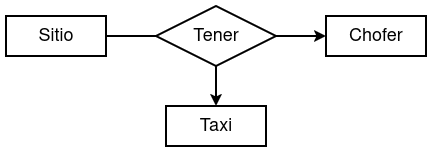
\includegraphics[width=0.6\textwidth]{imagenes/a)Restricciones.png}
        \caption{Diagrama actualizado con las restricciones correspondientes.}
    \end{figure}
\end{enumerate}
